\documentclass[10pt]{article}
\usepackage[ngerman]{babel}
\usepackage[utf8]{inputenc}
\usepackage[T1]{fontenc}
\usepackage{graphicx}
\usepackage[export]{adjustbox}
\graphicspath{ {./images/} }
\usepackage{hyperref}
\hypersetup{colorlinks=true, linkcolor=blue, filecolor=magenta, urlcolor=cyan,}
\urlstyle{same}

\begin{document}
\section*{WBE: UI-BIBLIOTHEK}
 TEIL 1: KOMPONENTEN\section*{ÜBERSICHT}
\begin{itemize}
  \item Frameworks und Bibliotheken
  \item DOM-Scripting und Abstraktionen
  \item JSX und SJDON
  \item Eigene Bibliothek: SuiWeb
\end{itemize}

\section*{ÜBERSICHT}
\begin{itemize}
  \item Frameworks und Bibliotheken
  \item DOM-Scripting und Abstraktionen
  \item JSX und SJDON
  \item Eigene Bibliothek: SuiWeb
\end{itemize}

\section*{BIBLIOTHEK}
\begin{itemize}
  \item Kontrolle beim eigenen Programm
  \item Funktionen und Klassen der Bibliothek verwendet
  \item Beispiel: jQuery\\
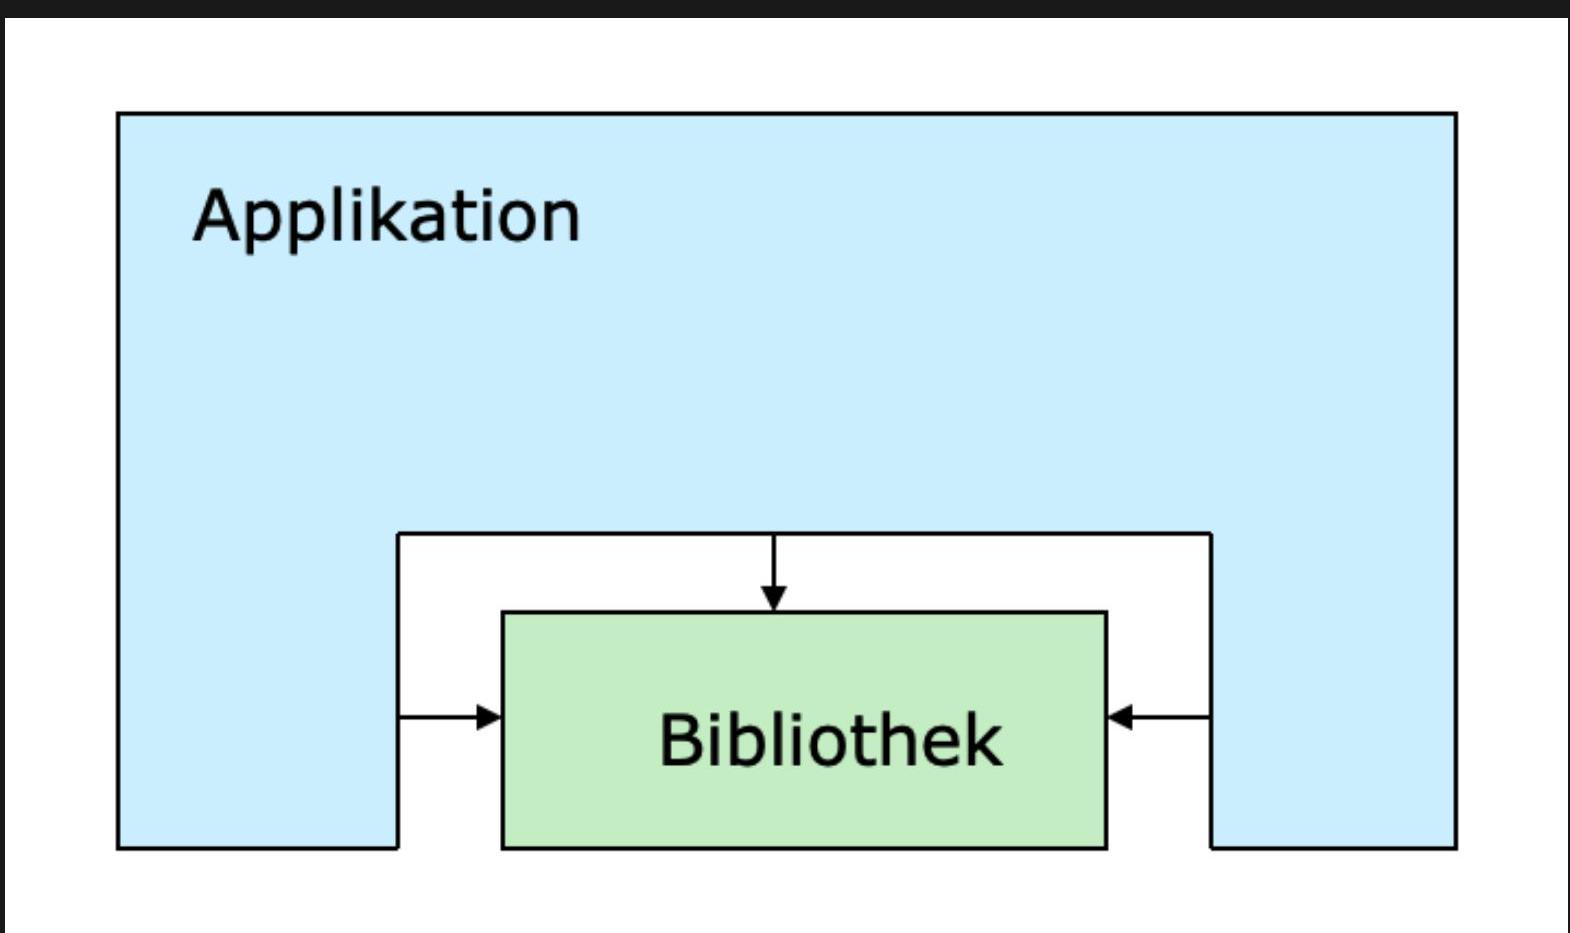
\includegraphics[width=\linewidth]{images/2025_01_02_22162ee5453ad0230328g-04}
\end{itemize}

\section*{FRAMEWORK}
\begin{itemize}
  \item Rahmen für die Anwendung
  \item Kontrolle liegt beim Framework
  \item Hollywood-Prinzip: „don't call us, we'll call you"\\
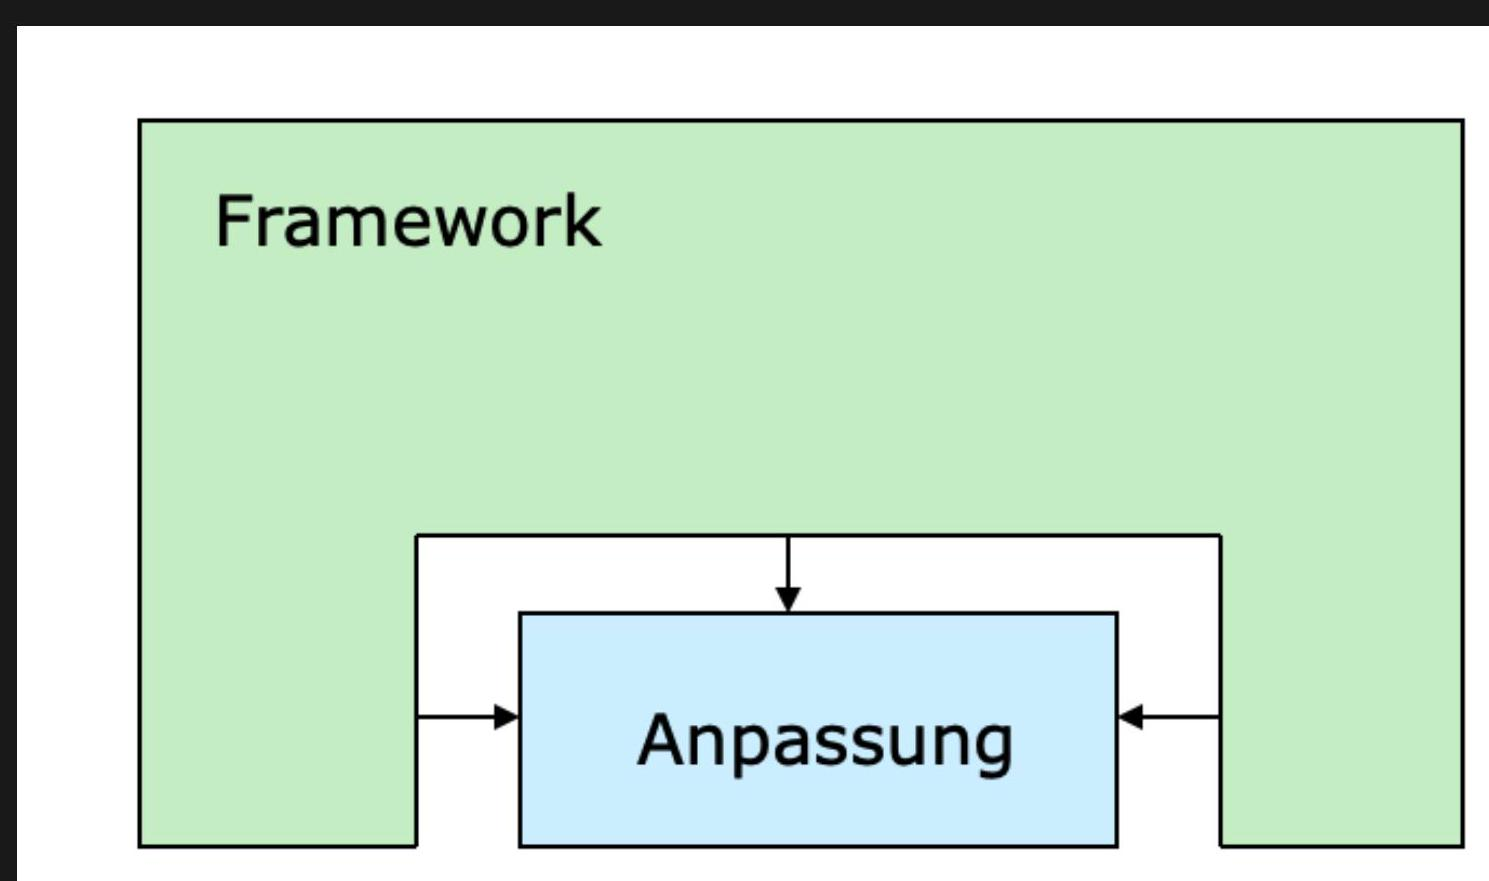
\includegraphics[width=\linewidth]{images/2025_01_02_22162ee5453ad0230328g-05}
\end{itemize}

\section*{ANSÄTZE IM LAUF DER ZEIT}
\begin{itemize}
  \item Statische Webseiten
  \item Inhalte dynamisch generiert (CGI z.B. Shell Scripts, Perl)
  \item Serverseitig eingebettete Scriptsprachen (PHP)
  \item Client Scripting oder Applets (JavaScript, Java Applets, Flash)
  \item Enterprise Application Server (Java, Java EE)
  \item MVC Server-Applikationen (Rails, Django)
  \item JavaScript Server (Node.js)
  \item Single Page Applikationen (SPAs)
\end{itemize}

\section*{SERVERSEITE}
\begin{itemize}
  \item Verschiedene Technologien möglich
  \item Zahlreiche Bibliotheken und Frameworks
  \item Verschiedene Architekturmuster
  \item Häufig: Model-View-Controller (MVC)
  \item Beispiel: Ruby on Rails
\end{itemize}

\section*{MODEL-VIEW-CONTROLLER (MVC)}
Models

\begin{itemize}
  \item repräsentieren anwendungsspezifisches Wissen und Daten
  \item ähnlich Klassen: User, Photo, Todo, Note
  \item können Observer über Zustandsänderungen informieren
\end{itemize}

\section*{Views}
\begin{itemize}
  \item bilden die Benutzerschnittstelle (z.B. HTML/CSS)
  \item können Models überwachen, kommunizieren aber normalerweise nicht direkt mit innen
\end{itemize}

\section*{Controllers}
\begin{itemize}
  \item verarbeiten Eingaben (z.B. Clicks) und aktualisieren Models
\end{itemize}

\section*{RUBY ON RAILS}
\begin{itemize}
  \item Serverseitiges Framework, basierend auf MVC
  \item Programmiersprache: Ruby\\
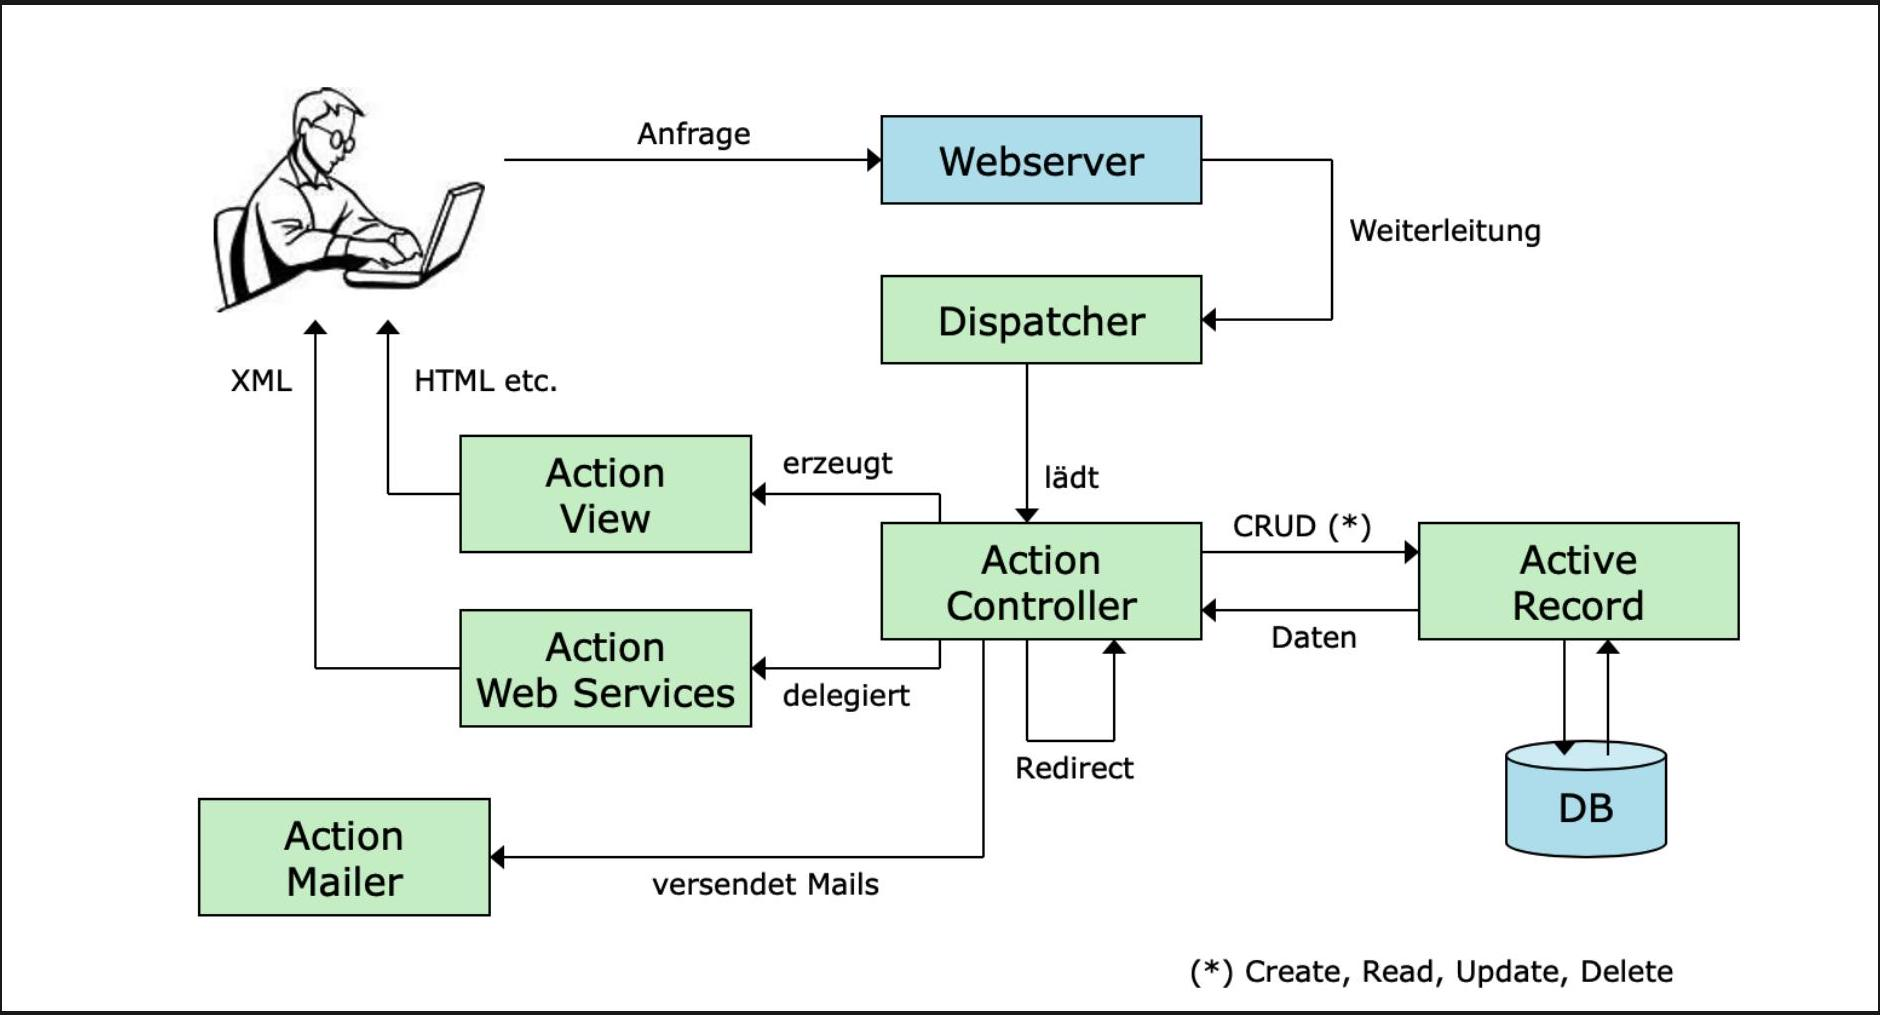
\includegraphics[width=\linewidth]{images/2025_01_02_22162ee5453ad0230328g-09}
\end{itemize}

\section*{"Convention over Configuration"}
\href{https://rubyonrails.org}{https://rubyonrails.org}

\section*{FOKUS AUF DIE CLIENT-SEITE}
\begin{itemize}
  \item Programmlogik Richtung Client verschoben
  \item Zunehmend komplexe User Interfaces
  \item Asynchrone Serveranfragen, z.B. mit Fetch
  \item Gute Architektur der Client-App wesentlich
  \item Diverse Frameworks und Bibliotheken zu diesem Zweck
\end{itemize}

\section*{SINGLE PAGE APPS (SPAs)}
\begin{itemize}
  \item Neuladen von Seiten vermeiden
  \item Inhalte dynamisch nachgeladen (Ajax, REST)
  \item Kommunikation mit Server im Hintergrund
  \item Ul reagiert schneller (Usability)
\end{itemize}

\section*{ÜBERSICHT}
\begin{itemize}
  \item Frameworks und Bibliotheken
  \item DOM-Scripting und Abstraktionen
  \item JSX und SJDON
  \item Eigene Bibliothek: SuiWeb
\end{itemize}

\section*{DOM-SCRIPTING}
\begin{itemize}
  \item Zahlreiche Funktionen und Attribute verfügbar
  \item Programme werden schnell unübersichtlich
  \item Gesucht: geeignete Abstraktionen
\end{itemize}

\section*{AUFGABE}
\begin{itemize}
  \item Zum Vergleich der verschiedenen Ansätze
  \item Liste aus einem Array erzeugen
\end{itemize}

\begin{verbatim}
/* gegeben: */
let data = ["Maria", "Hans", "Eva", "Peter"]
<!-- DOM-Struktur entsprechend folgendem Markup aufzubauen: -->
<ul>
    <li>Maria</li>
    <li>Hans</li>
    <li>Eva</li>
    <li>Peter</li>
</ul>
\end{verbatim}

\section*{DOM-SCRIPTING}
\begin{verbatim}
function List (data) {
    let node = document.createElement("ul")
    for (let item of data) {
        let elem = document.createElement("li")
        let elemText = document.createTextNode(item)
        elem.appendChild(elemText)
        node.appendChild(elem)
    }
    return node
}
\end{verbatim}

\begin{itemize}
  \item Erste Abstraktion: Listen-Komponente
  \item Basierend auf DOM-Funktionen
\end{itemize}

\section*{DOM-SCRIPTING}
\begin{verbatim}
function init () {
    let app = document.querySelector(".app")
    let data = ["Maria", "Hans", "Eva", "Peter"]
    render(List(data), app)
}
function render (tree, elem) {
    while (elem.firstChild) { elem.removeChild(elem.firstChild) }
    elem.appendChild(tree)
}
\end{verbatim}

\section*{DOM-SCRIPTING VERBESSERT}
\begin{verbatim}
function elt (type, attrs, ...children) {
    let node = document.createElement(type)
    Object.keys(attrs).forEach(key => {
        node.setAttribute(key, attrs[key])
    })
    for (let child of children) {
        if (typeof child != "string") node.appendChild(child)
        else node.appendChild(document.createTextNode(child))
    }
    return node
}
\end{verbatim}

\section*{DOM-SCRIPTING VERBESSERT}
\begin{itemize}
  \item Damit vereinfachte List-Komponente möglich
  \item DOM-Funktionen in einer Funktion elt gekappselt
\end{itemize}

\begin{verbatim}
function List (data) {
    return elt("ul", {}, ...data.map(item => elt("li", {}, item)))
}
\end{verbatim}

\section*{JQUERY}
\begin{verbatim}
function List (data) {
    return $("<ul>").append(...data.map(item => $("<li>").text(item)))
}
function render (tree, elem) {
    while (elem.firstChild) { elem.removeChild(elem.firstChild) }
    $(elem).append(tree)
}
\end{verbatim}

\begin{itemize}
  \item List gibt nun ein jQuery-Objekt zurück
  \item Daher ist eine kleine Anpassung an render erforderlich
\end{itemize}

\section*{WEB COMPONENTS}
\begin{itemize}
  \item Möglichkeit, eigene Elemente zu definieren
  \item Implementiert mit HTML, CSS und JavaScript
  \item Implementierung im Shadow DOM verstecken
\end{itemize}

\begin{verbatim}
<custom-progress-bar class="size">
<custom-progress-bar value="25">
<script>
    document.querySelector('.size').progress = 75;

\section*{REACT.JS}
\end{verbatim}

const List = (\{data\}) => (\\
\\
\{ data.map(item => (\{item\})) \}\\
\\
)\\
const root = createRoot(document.getElementById('app'))\\
root.render(\\[0pt]
<List data=\{["Maria", "Hans", "Eva", "Peter"]\} />\\
)

\begin{verbatim}
- XML-Syntax in JavaScript: JSX
- Muss zu JavaScript übersetzt werden
- https://reactjs.org

\section*{VUE.JS}
\end{verbatim}

\begin{verbatim}
https://vuejs.org
\end{verbatim}

var app4 = new Vue(\{\\
el: '\#app',\\
data: \{\\
items: [\\
\{ text: 'Learn JavaScript' \},\\
\{ text: 'Learn Vue' \},\\
\{ text: 'Build something awesome' \}\\[0pt]
]\\
\}\\
\})

\begin{verbatim}

\section*{ÜBERSICHT}
- Frameworks und Bibliotheken
- DOM-Scripting und Abstraktionen
- JSX und SJDON
- Eigene Bibliothek: SuiWeb

\section*{EIGENE BIBLIOTHEK}
- Ziel: eigene kleine Bibliothek entwickeln
- Ideen von React.js als Grundlage
- In dieser und den folgenden Lektionen schrittweise aufgebaut
- Wir nennen es:

\author{
SuiWeb \\ Simple User Interface Toolkit for Web Exercises
}

\section*{EIGENE BIBLIOTHEK: MERKMALE}
![](https://cdn.mathpix.com/cropped/2025_01_02_22162ee5453ad0230328g-25.jpg?height=1024&width=891&top_left_y=856&top_left_x=243)
- Komponentenbasiert
- Also: User Interface aus Komponenten zusammengesetzt
- Zum Beispiel:

Komponente ArticleList

\section*{EIGENE BIBLIOTHEK: MERKMALE}
![](https://cdn.mathpix.com/cropped/2025_01_02_22162ee5453ad0230328g-26.jpg?height=1101&width=704&top_left_y=813&top_left_x=241)
- Datengesteuert
- Input: Daten der Applikation
- Output: DOM-Struktur für Browser

\section*{(data) =>}
![](https://cdn.mathpix.com/cropped/2025_01_02_22162ee5453ad0230328g-27.jpg?height=547&width=838&top_left_y=951&top_left_x=1901)

\section*{NOTATION FÜR KOMPONENTEN}
- Gesucht: Notation zum Beschreiben von Komponenten
- Ziel: möglichst deklarativ
- Also nicht: imperativen JavaScript- oder jQuery-Code, der DOM manipuliert
- Verschiedene Möglichkeiten, z.B.
- JSX: in React.js verwendet
- SJDON: eigene Notation
\end{verbatim}

JSX\\
const Hello = () => (\\
Hello World\\
)

\begin{verbatim}
- Von React-Komponenten verwendete Syntax
- Komponente beschreibt DOM-Struktur mittels JSX
- HTML-Markup gemischt mit eigenen Tags
- JSX = JavaScript XML
(oder: JavaScript Syntax Extension?)

\section*{JSX INS DOM ABBILDEN}
\end{verbatim}

const domNode = document.getElementById('app')\\
const root = createRoot(domNode)\\
root.render()

\begin{verbatim}
- Root zum Rendern der Komponente anlegen
- Methode render aufrufen mit Code der gerendert werden soll

\section*{JSX}
- Problem: das ist kein JavaScript-Code
- Sondern: JavaScript-Code mit XML-Teilen
- Muss erst in JavaScript-Code übersetzt werden (Transpiler)
- Browser erhält pures JavaScript
![](https://cdn.mathpix.com/cropped/2025_01_02_22162ee5453ad0230328g-31.jpg?height=780&width=2082&top_left_y=1399&top_left_x=222)

\section*{JSX: HTML-ELEMENTE}
- HTML-Elemente als vordefinierte Komponenten
- Somit können beliebige HTML-Elemente in Komponenten verwendet werden
\end{verbatim}

root.render(\\


A Header

\\
)

\begin{verbatim}

\section*{JSX: HTML-ELEMENTE}
- HTML-Tags in Kleinbuchstaben
- Eigene Komponenten mit grossen Anfangsbuchstaben
- HTML-Elemente können die üblichen Attribute haben
- Wenige Ausnahmen, z.B.:
class-Attribut heisst className in JSX

\section*{JSX: KOMPONENTEN}
\end{verbatim}

1 const MyComponent = () => (\\

My Component
Content in my component...
\\
)\\
root.render(\\
\\
10 )

\begin{verbatim}

\section*{JSX: KOMPONENTEN}
\end{verbatim}

const List = (\{data\}) => (\\
\\
\{ data.map(item => (\{item\})) \}\\
\\
)\\
root.render(\\[0pt]
<List data=\{["Maria", "Hans", "Eva", "Peter"]\} />\\
)

\begin{verbatim}
- JavaScript in JSX in \{... \}

\section*{JSX: KOMPONENTEN}
- Funktionen, welche JSX-Code zurückgeben
- Neue Komponente kann dann als Tag im JSX benutzt werden
- Üblicherweise werden Komponenten in eigenen Modulen implementiert und bei Bedarf importiert

\section*{SJDON}
- Alternative zu JSX, eigene Notation
- SJDON - Simple JavaScript DOM Notation
- Bezeichnung aus einer Semesterendprüfung in WWD (WebPublishing und Webdesign, G. Burkert, 2011 an der ZHAW)
4. JavaScript-Datenstrukturen, JSON, PHP (12 Punkte)

In einer Ajax-Anwendung soll HTML-Code in einfachen JavaScript-Datenstrukturen aufgebaut und manipuliert werden. Diese können dann im JSON-Format an den Server übertragen und zum Beispiel in einer Datenbank gespeichert werden. Schliesslich lässt sich aus den Strukturen auf relativ einfache Weise wieder HTML-Code generieren.

Die Notation - nennen wir sie SJDON (Simple JavaScript DOM Notation) - sei wie folgt definiert:

Die Notation - nennen wir sie SJDON (Simple JavaScript DOM Notation) - sei wie folgt definiert:
- Ein Textknoten ist einfach der String mit dem Text.
- Ein Elementknoten ist ein Array, das als erstes den Elementnamen als String enthält und anschliessend die Kindelemente (Text- oder Elementknoten, in der gewünschten Reihenfolge) und Attributbeschreibungen für den Elementknoten.
- Attributbeschreibungen sind Objekte deren Attribute und Werte direkt den Attributen und Werten des HTML-Elements entsprechen. Alle Attribute des Elements können in einem Objekt zusammengefasst oder auf mehrere Objekte verteilt werden.
![](https://cdn.mathpix.com/cropped/2025_01_02_22162ee5453ad0230328g-38.jpg?height=919&width=2313&top_left_y=1119&top_left_x=647)

\section*{VERGLEICH}
\end{verbatim}

/* JSX \textit{/\\
const element = (\\

Hello World
from SuiWeb
\\
)\\
/} SJDON */\\
const element =\\[0pt]
["div", \{style: "background:salmon"\},\\[0pt]
["h1", "Hello World"],\\[0pt]
["h2", \{style: "text-align:right"\}, "from SuiWeb"] ]

\begin{verbatim}

\section*{ELEMENTE}
- Ein Element wird als Array repräsentiert
- Das erste Element ist der Elementknoten
- String: DOM-Knoten mit diesem Typ
- Funktion: Selbst definierte Komponente
\end{verbatim}

["br"] /* br-Element \textit{/\\[0pt]
["ul", ["li", "eins"], ["li", "zwei"]] /} Liste mit zwei Items \textit{/\\[0pt]
[App, \{name: "SuiWeb"\}] /} Funktionskomponente */

\begin{verbatim}

\section*{ATTRIBUTE}
- Als Objekte repräsentiert
- Irgendwo im Array (ausser ganz vorne)
- Mehrere solcher Objekte werden zusammengeführt
\end{verbatim}

/* mit style-Attribut, Reihenfolge egal */\\[0pt]
["p", \{style: "text-align:right"\}, "Hello world"]\\[0pt]
["p", "Hello world", \{style: "text-align:right"\}]

\begin{verbatim}

\section*{FUNKTIONEN}
- Funktion liefert SJDON-Ausdruck
- Kein \{ . . . \} für JavaScript wie in JSX nötig
\end{verbatim}

const App = (\{name\}) =>\\[0pt]
["h1", "Hi ", name]\\
const element =\\[0pt]
[App, \{name: "SuiWeb"\}]

\begin{verbatim}

\section*{BEISPIEL: LISTENKOMPONENTE}
\end{verbatim}

const MyList = (\{items\}) =>\\[0pt]
["ul", ...items.map(item => ["li", item]) ]\\
const element =\\[0pt]
[MyList, \{items: ["milk", "bread", "sugar"]\}]

\begin{verbatim}
- JavaScript-Ausdruck generiert Kind-Elemente für ul
- Kein Problem, JavaScript-Ausdrücke einzufügen SJDON is pure JavaScript ;)

\section*{ÜBERSICHT}
- Frameworks und Bibliotheken
- DOM-Scripting und Abstraktionen
- JSX und SJDON
- Eigene Bibliothek: SuiWeb

\section*{ZIEL}
- Bau einer kleinen Web-Bibliothek
- Ausgerichtet an den Ideen von React
- Komponenten in JSX oder SJDON

\author{
Motto: \\ Keep it simple
}

\section*{SuiWeb}
- Simple User Interface Toolkit for Web Exercises
- Kein Mega-Framework
- Keine "full-stack"-Lösung
- Daten steuern Ausgabe der Komponenten
- Komponenten können einen Zustand haben

\section*{KEIN TWO-WAY-BINDING}
![](https://cdn.mathpix.com/cropped/2025_01_02_22162ee5453ad0230328g-47.jpg?height=365&width=1843&top_left_y=750&top_left_x=408)
- Ul-Elemente nicht bidirektional mit Model-Daten verbunden
- Daten werden verwendet, um View zu generieren
- Benutzerinteraktionen bewirken ggf. Anpassungen am Model
- Dann wird die View erneut aus den Daten generiert

\section*{AUSBLICK}
- Schrittweiser Aufbau von SuiWeb
- Beispiele im Praktikum

Wichtiger Hinweis: React.js ist ein bekanntes und verbreitetes Framework und JSX eine bekannte Notation. SJDON und SuiWeb sind eigene Entwicklungen und ausserhalb WBE unbekannt...

\section*{QUELLEN}
- React - A JavaScript library for building user interfaces https://reactjs.org
- Adam Boduch: React and React Native Second Edition, Packt Publishing, 2018 Packt Online Shop

\section*{JSX UND ALTERNATIVEN}
- Draft: JSX Specification https://facebook.github.io/jsx/
- Babel - a JavaScript compiler http://babeljs.io
- Eigene Notation: SJDON https://github.com/gburkert/sjdon

Alternativen:
- HyperScript - Create HyperText with JavaScript https://github.com/hyperhype/hyperscript
- Hiccup - library for representing HTML in Clojure https://github.com/weavejester/hiccup

\section*{Stand:}
12.11.2024 12:44
\end{verbatim}


\end{document}